
\chapter{General Information about RFID technology}
\label{Kap2}

\section{General Information}

According to Ajami and Rajabzadeh \cite{ncbi} RFID technology is capable of an automatic unambiguous identifiation without being placed in the line of sight of their objects. The data between RFID tags and readers is transmitted through radio waves. In the 1940ies, the technology was firstly used to identify airplanes during war. Today, it is used in several different areas, like for example in manufacturing, supply chains, agriculture, transportation systems, healthcare services etc. 

\subsection{Components of an RFID application}

Ajami and Rajabzadeh \cite{ncbi} mention five main components existing in a RFID system. Firstly, there is the RFID tag attached to an object ensuring its unique identification. Secondly, the has to be an antenna which detects each tag and creates a magnetic field. The antenna is connected to its reader which receives the tag's information and is able to manipulate tags. Thirdly, in every RFID system has to exist a communication infrastructure which enables the interaction of readers and tags through an \ac{IT} infrastructure. Lastly, to enable users to connect to the RFID infrastructure and to control its modules, there has to be established a application software, such as a database or user interface.

\subsubsection{RFID tags} \label{tags}

Henrici \cite{henrici} states that there are two types of RFID tags: Tags with 'Smartcard'-like functionality and 'Auto-id' systems. The first type of RFID tag  provides extended functionalities and has computational capabilities. Furthermore, sensors can be attached to the 'Smartcard'-like tags which measure and control temperature and can be used for telemetry applications. In contrast, the 'Auto-id' systems imply the automatic identification of its objects. Generally spoken, RFID systems can be seen as a subset of 'Auto-id' systems.

When it comes to the variety of RFID tags, three fundamental types are distinguished: Active, semi-active and passive RFID tags \cite{henrici} which all constist of an antenna, a microchip and packaging. Active RFID tags consist of a microchip and have their own power source. As a characteristic, they are more expensive than the other two types. After that, semi-active tags or also called 'hybride' tags have their own power supply which is only used to support the microchip. The transmission or communication between semi-active tag and reader is implemented by using the power of the reader's field. Lastly, the passive RFID tags do not consist of a power source and only work in the reading range of the reader. They harvest their needed energy from the electromagnetic field of the reader and are cheaper than active tags. Moreover, passive tags are lighter than active tags and provide a long-lasting service. In constrast to active tags, passive tags are limited in their read range and functionality.

According to Henrici \cite{henrici}, the memory capacity of passive RFID tags can vary from single bits to kilobytes which is not much. As a recommendation, an external database to store tag-specific data should be used. For instance, a memory of 12 byte is very common to store \ac{EPC}. Concerning the memory technology, Henrici distinguishes two general types of storage: non-volatile and volatile storage. Non-volatile storage can be divided into read-only (fixed after manufacturing), \ac{WORM} and read-write which set the access privileges to the memory. The opposite of non-volatile storage is called volatile storage and is used for example to perform calculations after power-up. Besides, Henrici mentions tags which check passwords or implement ciphering algorithms to ensure data privacy. To visualize the tag's data and to provide real-time measurement, passive tags can be equipped with displays, buttons and temperature sensors. 

To maintain the security and authenticity of each RFID tag, Henrici \cite[p.93 ff.]{henrici} depicts four implementation methods of identification. 
The first and easiest method is called 'regular identification'. It implies that each tag sends its complete identifier to the reader within a \ac{SMLE}. Another method is called 'implicit identification'. It uses information that has not been provided explicitly for particular identification purpose. Thirdly, a more complexe and secure method to identify tags which is called 'multistep identification' is described by Henrici. As the name of this method is very self-explaining, one has to think of three identification steps: In the first step, only parts of the identification information is revealed. After that, an authentication and authorization step follows. Once, being authenticated and authorized, more identification information will be revealed. 
Other than the mentioned methods, Henrici describes a fourth and most secure method to identify tags which he calls 'encryption and shared key identification'. As an advantage, this identification method protects every information contained in an identifier which can be transmitted in encrypted form. The vast amount of information requires a high internal storage of the tag, like given by active tags. To arrange an encrypted tranmission of information from passive, low cost tags the identifier needs to be calculated outside the tag and then stored on the tag (directly in enciphered form). So, it would be no additional expenditure to enable encrypted and shared key identification of tags using passive tags. 

\begin{figure}
\centering
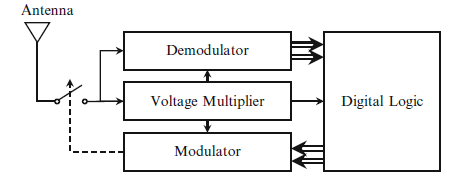
\includegraphics[width=\textwidth]{rfidtagdesign} The design of RFID tags 
\caption{\label{fig:tagdesign}The adopted from \cite[p.13]{chipless}} 
\end{figure}

\subsubsection{RFID readers} \label{reader}

In this section, RFID readers will be explained in detail. To start with, one has to imagine existing objects which are tagged with a RFID tag. To implement functionality to these tags and to connect them to a middleware or a backend system, a detector is needed. This detector is the RFID reader and consists of an antenna, a power supply for passive tags, a microprocessor (to control devices) and an interface for forwarding data to the processing backend system \cite{henrici}. 
Generally, two different types of readers can be distinguished: Stationary and mobile readers. To give an example of the use of stationary readers, they can be used for goods receiving or stock management. Furthermore, stationary readers are fixed to a specific location and need permanent network connection. On the opposite, mobile readers do not need permanent network connection and are used for querying prices in a supermarket.
As mentioned in the section before \pageref{tags}, RFID tags and readers communicate via electromagnetism. The reader's detection range depends on the frequency as well as the electromagnetic field \cite{henrici}. In general, four frequency ranges can be differenced: \ac{LF} (125-134 kHz),\ac{HF}(13,56 MHz), \ac{UHF} (868 MHz-915 MHz) and Microwave (2,54 GHz-5,8 GHz). Each frequency range has its own physical characteristics, such as the needed size of antennas or the read range.
According to Vizinex \cite{vizinex}, an american company with site in Pennsylvania, U.S HF tags can be used for short read ranges (up to 3 inches). They are usually tagged to tissue samples, blood and critical fluids. Furthermore, HF tags work well in proximidity to liquids as well as human tissues. UHF tags provide longer read ranges and can be detuned by proximity to tissue, fluids and metals. These tags are typically used to track and locate critical medical devices, manage inventories of medical items and track as well as identify patients. Moreover, UHF tags are compatible with worldwide standards and easily deployed because of the compatibility with widely available and competitively priced RFID readers.
Furthermore, each reader has its own electromagnetic field. Such fields are distinguished into near field and far fields: Near fields, also called magnetic or electric fields work with induction and capacitive coupling whereas far fields consist of electromagnetic waves. The measuring unit of electromagnetic fields is called field strength and the maximal field strength depends on national regulations. These national regulations limit the electromagnetic compatibility to avoid disturbing other systems. The functionality of passive tags within near field is different from passive tags in far field. In near field, the tags send data to the reader using load modulation. This mechanism does not work in far fields: Here, the sended frequency is backscattered \cite{henrici}.
All in all, readers are able to query tags and to read and write tag data. But the storage of information and the information processing does not take place in readers or tags, but in the middleware or backend systems. These will be explained in the following paragraph.

\begin{figure}
\centering
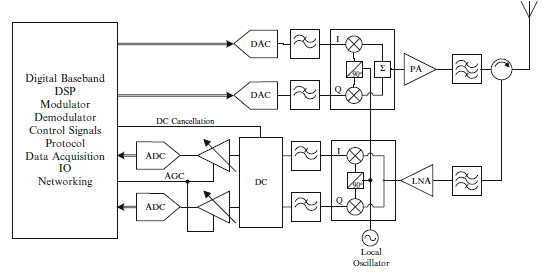
\includegraphics[width=\textwidth]{rfidreaderdesign} The design of a RFID reader 
\caption{\label{fig:readerdesign}The adopted from \cite[p.17]{chipless}} 
\end{figure}

\subsubsection{RFID backend systems} \label{backend}

As Henrici \cite{henrici} mentions, the backend can be divided into two parts: Middleware and applications. Both of them run on the same computer within the same network which is important for the permanent connection to RFID readers and all existing tags. The advantages of a middleware in this use are that no adaption of appications is needed, an open and neutral interface for other applications is provided. Besides, as the middleware is used to aggregate and filter data the processing is moved from tags into middleware so that tags only have to identify objects. As a result, modularity of the system is maintained.

Concerning the data management of RFID systems, data is barely stored on RFID tags because of the limited resources in low-cost tags. It is recommended \cite{henrici} to store tag information on an encapsulated database. As an advantage, databases provide high flexibility to change data or to execute queries without the tags being present. Furthermore, the backend infrastructure should use a \ac{SSL} or \ac{TLS} protocol to ensure a secure transmission of data. Finally, the data would be transmitted and stored in a backend infrastructure on a central storage \cite{henrici}.

\subsection{Functionality of RFID system}

First of all, when developing an RFID system, it is important to think about the unique identification of each object. To enable a reliable identification of objects, only one RFID tag should be attached to each object. The tag itself has a 'read-only' or in some cases 'rewrite' internal memory which enables users to get or change the object's information \cite{ncbi}. 
Secondly, the RFID reader generates magnetic fields to enable the RFID system to locate objects (via tags) within its range. Additionally, the high-frequency electromagnetic energy and the query signal which is generated by the reader triggers tags to reply to the query. Each query can have a frequency of 50 times per second \cite{ncbi}. Thus, it is possible to generate large quantities of data which have to be filtered by supply chain industries. Each filter is routed to a backend information system, using a software similar to 'Savant' which is used to control the data. 'Savant' acts like a buffer between the \ac{HIS} and the RFID reader \cite{ncbi}.

\subsection{Chipless RFID systems}

Rezaiesarlak et al. \cite[p.17]{chipless}

\begin{figure}
\centering
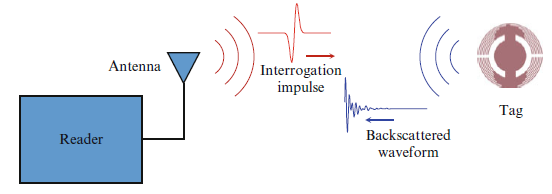
\includegraphics[width=\textwidth]{chipless_architecture} The architecture of chipless RFID systems 
\caption{\label{fig:chipless_architecture}The adopted from \cite[p.19]{chipless}} 
\end{figure}

\begin{figure}
\centering
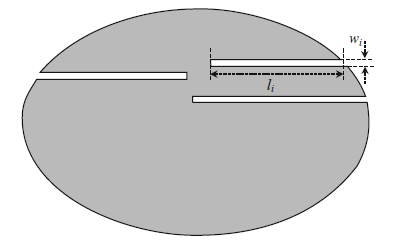
\includegraphics[width=\textwidth]{chiplesstag} The design of chipless RFID tags 
\caption{\label{fig:chipless_tag}The adopted from \cite[p.19]{chipless}} 
\end{figure}

\begin{figure}
\centering
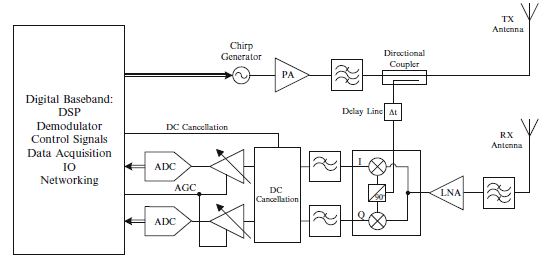
\includegraphics[width=\textwidth]{chiplessreader} The design of chipless RFID readers 
\caption{\label{fig:chipless_reader}The adopted from \cite[p.20]{chipless}} 
\end{figure}

\subsection{Security and Privacy of RFID systems}

Security and privacy in the healthcare sector is a very important and highly discussed issue. As these are very large issues, which could not be described within a few paragraphs, there will be depicted some examples of threats. In the second section 'Solutions and Methods against Threats' \pageref{solution}, five important recommended countermeasures will be described.

\subsubsection{Security Problems and Threats} \label{problems}
 
As Henrici \cite{henrici} mentions, there exist two fundamental fears about the RFID technology. The first fear concerning marketing purposes, such as creating very detailed customer profiles which lead to a vast amount of information. Secondly, the technology offers the possibility to keep people under surveillance which implies advantages and disadvantages. As an advantage, the patients' life gets more confortable and companies will be more productive. As a negative result, people's privacy is violated and the application's security is not addressed properly.
Aside from the two fears, Henrici describes several risks of RFID systems, such as the ease of disrupting the service which indicates data security and privacy problems. When talking about security, one should distinguish between security of systems and services and the security of data and information. The last point can only be ensured by secure systems \cite{henrici}. 
In the following, some security and privacy risks using RFID technologies will be explained. To start with, one should think of his passport and the data which is stored on it. The new passports have an internal RFID tag which enables readers nearby the passport to read out all data and to copy them as well. As mentioned in section \pageref{tags}, passive RFID tags are cheap, do not have their own power supply and can be read through a nearby reader. So, reading out the passport's data would not be very complex.
Moreover, Henrici mentions product counterfeiting in pharmaceuticals which can cause a lot of harm, like the death of patient's. Nevertheless, the drug market is bound to strong regulations, like for example through the \ac{FDA}. To detect and reduce product counterfeiting, RFID tags need to prove genuineness of original products to patients and should inhibit cloning them.

In his book, Henrici mentions six cases of possible attacks to RFID systems \cite[p.61 ff.]{henrici}. The first attack is called 'Illegitimate reading of data' and describes the possibility of side-channel attacks which use the communication protocol between passive tags and backend systems. As described in section 'RFID backend systems' \pageref{backend}, passive tags are used more often and are less expensive than active tags. Nevertheless, the vulnerability of synchronizing each tag with the backend system through a protocol enables attackers to bypass normal protocols so that they can readout all transmitted data.
The second possible attack, Henrici mentions, is called 'eavesdropping of data'. It is caused by the problem of the public and shared communication channel between readers and tags. Compared to 'illegitimate reading of data', everybody near enough the communication channel is able to eavesdrop the conversation because of the use of passive tags. Particularly the 'forward' channel from reader to tag has a stronger magnetic field than the opposite direction which makes it more easily being eavesdropped than the backed one. 
Thirdly, Henrici declares 'cloning or mimicking of tags' as a third threat. His definition of cloning a tag is restricted to creating an exact logical copy of an item which is not distinguishable from the original tag on the protocol level. There might exist some minor differences like the power consumption or time response but the replica cannot be detected with ordinary readers but only with appropriate equipment. The second term 'mimicking' defines the action of infiltrating incorrect data into the RFID system. To show an example, the location might be used for authentication of items. By mimicking a tag, the location can be manipulated and items might appear where they do not exist in reality.
Fourthly, 'recognition of objects' represents another possible threat of RFID systems. In particular, when persons have been detected, they can be used to explore customer habits. Or, in case of patients who wear implants, these might be recognized and the medical information stored on each implant might be abused. In general, each person who carries objects with affixed RFID tags, like wristwatches, shoes etc. might be recognized by an attacker.
Next, the possibility 'tracking of objects' should be considered carefully since tracking of persons can cause many privacy violations. Henrici distinguishes two types of tracking: The first one is called 'direct mapping' and refers to the tracking of RFID wristwatches or glasses. 'Direct mapping' is only possible when the distance between detector and tag is short and the do not exist many tags in one place. Failing that, other items might be tracked by detecting their constellations to each other. These constellations can lead to unwanted creation of movement profiles and the abuse of infrastructure for surveillance by a totalitarian government.
Lastly, Henrici defines the threat of 'causing malfunction' which means that attackers (after having abused one of the above mentioned possibilities) are able to render RFID system malfunctioning. This malfuncionting can be revealed by physical destruction or chemical treatment of tags.  

\subsubsection{Solutions and Methods against Threats} \label{solution}

First of all, data security should always be maintained by the RFID system. But what are the exact countermeasures to prevent an attack on an existing RFID system? When Henrici \cite[p.64 ff.]{henrici} talks about solutions and methods against security threats, he calls them 'Goals of Security and Privacy'. In his book, these goals refer to the possible attacks or threats mentioned in section 'Security Problems and Threats' \pageref{problems}. In the following, the countermeasures will be explained. 
'Illegitimate reading of data' can be prevented by controlling data access and ensuring data integrity in RFID systems. False data should be infiltrated because of illegitimate access.
'Eavesdropping of data' can be coped with implementing means for detection and recovering so that the system should keep running even if attackers try to put it out of service. Besides, the integrity of system should always be kept. Another strategy preventing eavesdropping is to maintain data security. Henrici defines a 'good' RFID system to be able to cope with illegitimate reading of data and to treat all the data confidentially.
'Cloning or mimicking of tags' which can be compared to counterfeiting can be prevented by using authenticity mechanisms to identify specific tags. Therefore, RFID tags that can prove their own authenticity should be preferred.
Unwanted 'recognition of objects' can be avoided by developing technical models that provide suitable trade-off of functions. If a function is not wanted by the user, e.g. to allow everyone in the surroundings to read out all RFID attached object, he can adjust this by defining different user roles and rights.

Regarding the realization of the above mentioned goals, there exist many challenges which have to be faced. Henrici \cite[p.66 ff.]{henrici} describes four general challenges which will be explained in the following paragraph. 
First of all, since there are different parties, like e.g. logistic companies and customers which have different needs, the developer has to meet all of their requirements. For instance, the different user needs might be realized by developing different views which depend on the particular user role.
Secondly, developing a secure RFID system is a multidisciplinary challenge \cite{henrici} including six different departments: Computer science (designing communication protocols and the middleware), electrical engineering (realizing the required functionality in hardware and physical layer of communication between tags and readers), mathematics (developing basic cryptographic primitives and theory of probabilities for different areas), economics (adapting the application's constraints imposed by laws of market and assessing real world applicability of approaches), social sciences (including user's requirements, such as privacy and usability) and law (maintaining a legislative basis among people and organizations).
Thirdly, there are more requirements to be faced than 'only' security and privacy, such as low costs or coping with few capabilities and resources. Besides, the enrollment of an RFID system, e.g. in a hospital with many distinctive departments, leads to an inter-organizational operation. To implement this inter-organizational operation, several standards have to be integrated. 
Last but not least, additional requirements have to be considered: Scalability of the system, dependability, low complexity of system, robustness, transparency and usability etc. Henrici claims, that the safeguards should not limit the read range and the speed of reading. Moreover, when using cryptographic primitives, migration paths should be considered.  

\subsection{State of the Art}

There exist many companies which develop \ac{RFID} solutions and applications. In this paragraph, three important medical companies which provide RFID solutions, will be presented.

\subsubsection{Dipole Company}

To start with the first company, in the following, the spanish company 'Dipole' \cite{dipole} will be depicted. 'Dipole RFID' was found in Barcelona 20 years ago with the aim of developing systems for intelligent identification, data capture and systems integration. In their product scope, Dipole provides three main products. The first product contains RFID as well as \ac{NFC} solutions which should improve optimizing processes, realizing industry 4.0 and the \ac{IoT}. The second product consists in manufacturing RFID tags to measure the according user needs of Dipole's users. The third product is composed of consulting services, RFID software and systems integration.
In their section 'RFID Hospital and Health', Dipole mentions some use cases for their RFID solutions. To give an example, the correct administration of banked blood can be controlled by using RFID tags. Or, when product stock or termination date of medication and drugs in a hospital have to be observed, RFID tags provide a simple and large-scale use instead of controlling the stock manually (which also brings the risk of human errors). For broader use in hospitals, such as managing whole buildings and improving their workflows, RFID solutions should be considered as well. There exist many hospitals which administrate their workflows with paper-based solutions. As a consequence, the processes are getting very slow and data is duplicated. Furthermore, the communication between several departments is flawed and causes further problems.
Another health service, provided by Dipole, is the 'Traceability of Analysis'. In a hospital or a healthcare institution, there are many processes which embody information about clinical analysis, blood tests and blood preservation. These information are very important for patient's diagnosis and treatment. In a laboratory, all tissue samples are stored and several cultivation processes have to be controlled. To increase efficiency of these processes, establishing a RFID system to track and identify all samples correctly would be a useful solution.
When it comes to the management of buildings and workflows, the asset tracking forms an important part. Dipole distinguishes two different classifications of assets: \ac{RTI} and products of high value, e.g. elements from the IT and mobile machines. The second type of elements needs specific control in real-time. For an appropriate tracking of IT elements it should be possible to locate each item in a global and detail view to be sure that it is settled in the correct place and under the right conditions, such as the correct temperature or low air humidity.
Another use case is guaranteeing the correct dosage of medication to patients which is very important for patient's health and and the work of nursing staff. To simplify the dosage of medication to each patient, RFID tags can be sticked to the pill cases to ensure the correct distribution in real-time. 
Concerning the management of patients, it is possible to track patients indiviually by wearing bracelets which contain a RFID tag. Currently, the tracking of persons is very controversial because the patient's privacy is offended by enabling his persecution. On the other side, RFID bracelets enable to register patient's actions in real-time and ensure their safety. For example, if a patient suffers from epilepsy, it is dificult to predict an epileptic shock. But if he wore a bracelet which constantly synchronizes his health status with the system, doctors would be able to act preventively against such shocks and could minimize his risk to die of his illness.
Not only managing whole buildings is important but also the tracking and control of material in the operating rooms plays a significant role. For instance, in operating room A exists a mobile \ac{CT} whereas operating room B only has set of instruments for surgery. When there is a emergency and the patient needs a CT because the doctor cannot say if he needs the suggested operation but in the operating room B does not exist a CT, it is necessary to detect the next mobile CT rapidly and not to deteriorate the patient's health status. 

\subsubsection{Cardinal Health Inc.} \label{inventory}

Cardinal Health Inc., with its headquarters in Dublin and Ohio, founded 100 years ago,  \cite{cardinal_web} is a global company which provides integrated healthcare services and products. There exist four product fields in the scope of Cardinal Health Inc.: logistics, caring of patients, business solutions, and guidance of patients.
Cardinal Health Inc. provides Inventory Management Solutions \cite{cardinal_video} which are specialized on hospital's inventory. In a promotional video, they quote different types of inventory systems, such as the '2-Bin-Kanban' system which is adapted for low cost items needing right sizing and bulk level. A second inventory system which provides management for low cost items needing oversight at the each level is the 'Barcode' system. For high value implantables and physician preference items, the company advertises RFID as best used technology. In the video \cite{cardinal_video}, they claim that reading RFID tags is fast, e.g. 100 tags can be read in seconds. Moreover, RFID tags implicate ease of use for users and support user's needs very quickly. The physician does not have to care about the data capture of his observation because all RFID tagged items are automatically tracked and the measured data is captured by backend interfaces which synchronize to other IT systems (like Materials Management System or Billing Systems). In addition to that, automatic data capture avoids redundant data entries, provides errors and saves time.
Another important fact about RFID technology is its accuracy and uniqueness. Cardinal Healthcare Inc. advertises that RFID applications enable automated real-time tracking at a unique item level. Beyond, these applications provide a pro-active management of expired and recalled products. As a result, RFID applications lead to a streamlined workflow in which charges are automatically captured for accurate billing and compliants as well as clinical documentation are supported. 
All in all, Cardinal Health Inc. claims that by using its Inventory Management Solution for hospitals will enable physicians and nurses to focus more on patient care and spend less time on managing supplies  \cite{cardinal_video}.

\subsubsection{Terso Solutions Inc.}

Terso Solutions Inc., formed in 2005 in Madison (Wisconsin, U.S.), is specialized on RFID product development and provides several \ac{RAIN} RFID solutions. RAIN RFID \cite{rainrfid} is a wireless technology which enables the wireless connection of items to the internet. As a global alliance, RAIN RFID promotes the universal adoption of \ac{UHF} RFID technology which can be compared to the WiFi Alliance. RAIN uses a standardized GS1 UHF Gen2 protocol to connect all members (network, software, readers, tags, items) of its solution.
However, Terso Solutions Inc. has developed a solution for Medical Field Inventory Tracking which prevents a wide range of services to hospitals. In a promo \cite{terso_video}, the company shows its solution which connects the RFID technology to medical field by integrating RFID into the medical kit. By using this Medical Field Inventory Tracking, sales can be instantly recorded, field inventories and reverse overstock situations can be run. Besides, automated inventory reporting is possible which brings the side benefit of eliminating shipping costs. Each wrap can be located by the system and the closest needed device is shown. The advantages that accrued are better handled recalls, eliminated overnight shipping demands and reduced expired products. All in all, Terso Solutions Inc. provides two large RFID applications: The 'RFID for Compliance and Product Integrity' and the 'RFID for Compliance and Implant Tracking' which have also been approved for case studies in two hospitals in the U.S.. The first hospital where Terso Solutions Inc. performed its 'TrackCore' case study was the North Kansas City Hospital. RAIN RFID-enabled intelligent cabinets, integrated with TrackCore Inc.'s tissue and implant tracking software as well as the 'TrackCore Operating Room' were tested. Furthermore, 'Jetstream', a cloud-based platform from Terso was proved at 'North Kansas City Hospital'. The second case study was implemented at St. Dominic Hospital. The tested application included Terso's autoated tissue and implant tracking solution using RFID.

\subsubsection{Vizinex RFID}

Vizinex RFID was founded in 2012 and is located in Bethlehem, Pennsylvania, U.S. Specialized on the development of RFID tags, Vizinex provides tracking, security and authentication solutions which are based on the RFID technology. Concerning RFID, the company mentions several use cases of the technology \cite{vizinex} which will be mentioned in the following. Firstly, RFID can be used to detect  counterfeited drugs. Secondly, the company suggests the use of RFID in the medical equipment field by establishing real time locating systems. As an example, hospital staff is able to rapidly locate critical medical devices, defibrillators. As a positive consequence, Vizinex remarks the enhancement of patient's safety and the reduction of investments in equipment which are needed \cite{vizinex}. Another use case is the inventory management (see also Cardinal Health Inc. \pageref{inventory}) and tracking of consumables used in an operation (like for example scalpels, sponges, clamps or surgical equipment). The last point (tracking of consumables in an operation) indicates that after each operation everything can be automatically accounted for. In respect of the use for patients, Vizinex instruct ID cards, wrist or ankle bands and labels which can be attached to patients records. The company declares these identification possibility as a great aid to ensure that the right procedures and medications are applied (see Chapter 1, Internal Communication \pageref{Kap1}). Regarding the possibility of patient tracking, Vizinex brings up patients with afflictions such as Alzheimer's disease which makes it very difficult to live securely alone. For that reason, tracking people which suffer from Alzheimer within a facility can improve and avoid the risks of getting lost or entering an area where these people might harm themselves. In regard to laboratories, Vizinex names the following examples. The RFID technology can be used to track tissue or fluid samples. While samples are moved through various preparation steps there can occur several errors from data entry or mishandling which can be avoided by automatic tracking. Consequently, the samples that arrive at the pathologist for analysis will automatically contain the related patient record. Besides, an indication can be called to the computer screen to ensure the proper association of the sample with the patient. 
As another example, Vizinex depict RFID uses for the discovery of drugs. Especially valuable assets are difficult to inventory but it is essential to do this with a high level of accuracy.
All in all, there exist many use cases for the RFID technology. Nevertheless, the use of this technology brings up some concern related to the confidentiality of medical information \cite{vizinex}. Vizinex calls RFID tags 'licence plates' for the items they tag because only the identification number is contained on the tag whereas all 'human readable' information (such as the asset, drug, tissue sample or patient) resides in a database. The FDA highly recommends the external storage of confidential and private patient data and proposes an outline of three components for ensuring medical information security \cite{vizinex}. First of all, all information should be kept confidential. Secondly, the data should be accurate and complete. Thirdly, the data should be available and accessible. To realize the third component, the information should be store on a computer based system. 
By maintaining these provisions, data entry errors will be reduced, work and information flows will be automated, asset and consumable inventories will be improved and the association of treatment plans with patients will be improved.